\documentclass{article}
\usepackage{tikz}
\usepackage{xcolor}

\definecolor{myblue}{RGB}{54,106,146}
\definecolor{bggray}{RGB}{240,240,240}

\begin{document}

\begin{center}
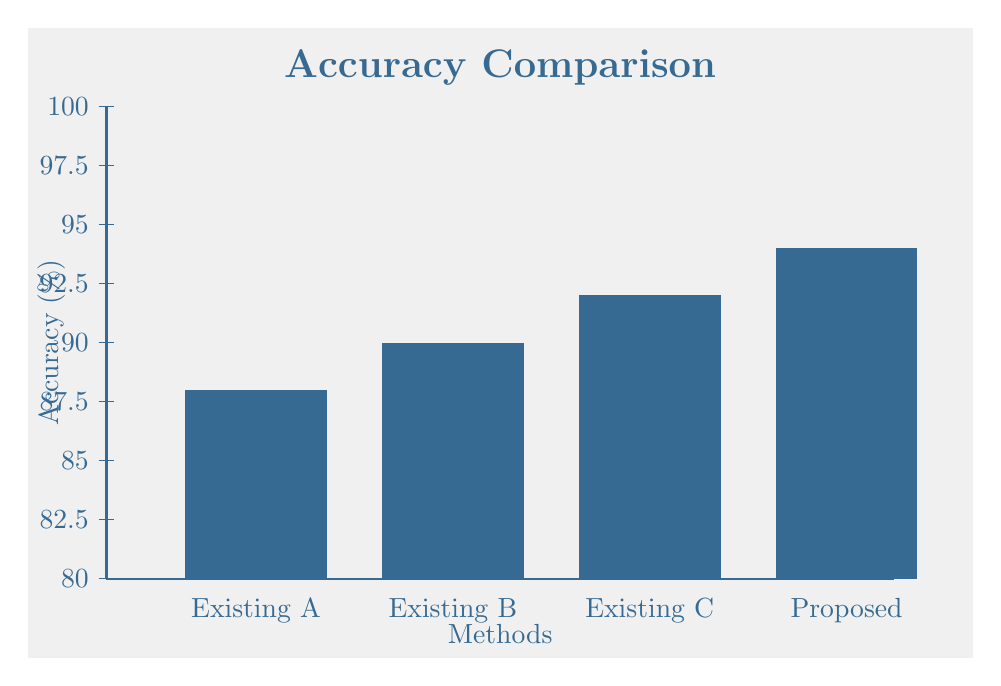
\begin{tikzpicture}

% Background
\fill[bggray] (0,0) rectangle (12,8);

% Axes
\draw[thick, myblue] (1,1) -- (1,7); % Y-axis
\draw[thick, myblue] (1,1) -- (11,1); % X-axis

% Title
\node[text=myblue, font=\Large\bfseries] at (6,7.5) {Accuracy Comparison};

% Labels
\node[rotate=90, text=myblue] at (0.3,4) {Accuracy (\%)};
\node[text=myblue] at (6,0.3) {Methods};

% Y-axis ticks (80 to 100)
\foreach \y/\val in {1/80,1.75/82.5,2.5/85,3.25/87.5,4/90,4.75/92.5,5.5/95,6.25/97.5,7/100} {
    \draw[myblue] (0.9,\y) -- (1.1,\y);
    \node[left, text=myblue] at (0.9,\y) {\val};
}

% Bars (scaled properly)
\def\scale{0.3}

\fill[myblue] (2,1) rectangle (3.8,{1 + (88-80)*\scale});
\fill[myblue] (4.5,1) rectangle (6.3,{1 + (90-80)*\scale});
\fill[myblue] (7,1) rectangle (8.8,{1 + (92-80)*\scale});
\fill[myblue] (9.5,1) rectangle (11.3,{1 + (94-80)*\scale});

% X labels
\node[text=myblue] at (2.9,0.6) {Existing A};
\node[text=myblue] at (5.4,0.6) {Existing B};
\node[text=myblue] at (7.9,0.6) {Existing C};
\node[text=myblue] at (10.4,0.6) {Proposed};

\end{tikzpicture}
\end{center}

\end{document}